\mysection{Downtime}{downtime}

Adventuring is both a risky and profitable endeavor. Your packs are filled with so much illegal wealth that they're about to burst open, and you've finally realized that the festering sore you got from the sentient vine needs to be examined by a specialist. Alternatively, you may have reached your limit of eating beetles that the Night Child had expelled. It's time to return to civilization for a break, to rest, recharge and enjoy some downtime.

Adventuring is both a dangerous and lucrative business. When your packs swell with enough ill gotten gains that they threaten to burst at the seams; when you finally decide that festering pustule you got from that sentient vine should probably be looked at by a professional; or when you simply can't eat another pile of beetles the Night Child vomited up it's time to head back to civilization for some rest, relaxation, and \mybold{Downtime}.

Downtime lasts for Days, Weeks, or Months and must take place in a Small, Medium, or Large Settlement (you can't take Downtime in a Tiny Settlement). You can rest for Days in a Small, Medium, or Large Settlement; for Weeks in a Medium or Large Settlement; and for Months in a Large Settlement without trouble. Staying Weeks or Months in a Small settlement could invite trouble, or at the very least the townsfolk will look at you as more than someone who is just "passing through"; same deal if you try to stay for Months in a Medium Settlement. 

Finally, an Adventurer can opt to take Downtime for Years (if they can afford it). If they do, they are considered to be retired from adventuring life.

\myfpimage{civilization/WallBreak}


\begin{multicols*}{2}

Downtime is divided into the following five steps:

\begin{center}
\fbox{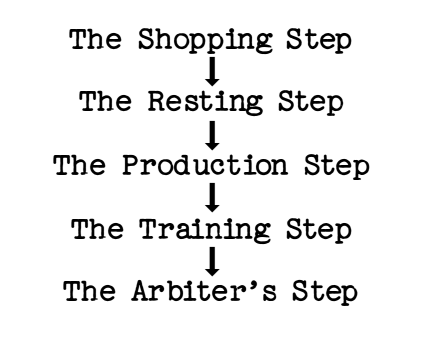
\includegraphics[width=.9\linewidth,keepaspectratio=true]{civilization/Downtime}}
\end{center}


\mybold{If there's no narrative purpose to role-playing any of these steps, just move through them in order and get back to your dungeon crawl}. However, if you wish to have additional interaction during any step, the Arbiter can play out a \mybold{Side Story}.


\mysubsection{Side Stories}{downtime-side-story}

Maybe you've been Geased to deliver a message to the Lich-Sultan of Zamora; or maybe those pesky assassin automata you thought were dead have tracked you to the city; or the Arbiter wants to use the optional rules for \mylink{A Spoonful Of...}{vulgate-medicine-crunch}.  These side stories can happen at any time during your Downtime, \mybold{but you only gain the benefits of the steps you've already completed}. For instance, if you wish to visit with the Lich-Sultan during the Shopping step, you haven't had a chance to take the Resting step and therefore you're not at full strength.  If the assassin automata decide to take you out in your second-floor rooms at the Inn of the Welcome Wrench during the Resting step, you are still unrested because you haven't completed the Resting step.

The longer you spend in a Settlement, the more it will cost you - but the more time you have to create items during the \mylink{Production}{downtime-production} step (see below). 

\mysubsection{The Shopping Step}{downtime-shopping}

First, you can sell the various tapestries, candelabra, spoons, hats, weird erotic cookbooks, etc. to discerning buyers. If you want to do some haggling, take a Side Story - otherwise the Arbiter will just tell you how much coin you've made. Note that sometimes something might not be sellable in the Settlement you're in (like trying to sell a Gaugin in a rural town) at the Arbiter's discretion. Again - if there's narrative purpose to the transaction, take a Side Story - otherwise, just convert to coin.

Second, you'll need to pay for lodging, food, "entertainment", healing supplies, drink, more drink, etc. depending on how long you're planning on staying in the Settlement (Days, Months, or Weeks).  Staying longer than Days increases the amount of \mylink{Research}{research} and \mylink{Cunning}{cunning} you can use during the Production step, provided the Settlement is large enough to accommodate your needs (see below).

\mytable{Y Y Y Y}{
    \thead{} & \thead{Small} & \thead{Medium} & \thead{Large}  \\
}{
    Days & 100 \FE & 50 \AG & 25 \AU \\
    Weeks & n/a & 200 \AG & 100 \AU  \\
    Months & n/a & n/a & 500 \AU  \\
    Years\footnote{\label{note1}taking Downtime for Years retires your Adventurer!} & n/a & n/a & 5,000 \AU \\
}
\callout {
    Taking Downtime for longer periods of time allows you to perform more complex actions with your Research and Cunning, or create more powerful magical blades.}

Finally, you can spend coin on any \mylink{Gear}{gear} you might want, including using \mylink{Services}{gear-services} like an Ironmonger to \mylink{repair your Armor}{gear-armor-repair}; a Mundunugu to remove a Curse; or a Chirugeon to heal a \mylink{Beating}{physical-wound-beating}, \mylink{Addiction}{gear-narcotics-addiction}, \mylink{Disease}, or Madness! Likewise, if you are practiced in the \mylink{Vulgate of Medicine}{vulgate-medicine}, you may use it during this step to cure Beatings, Addictions, and Diseases (but not Madness!).

\mysubsection{The Resting Step}{downtime-resting}

With all that commerce out of the way, you can now rest and recuperate in earnest. Unless a wound, curse, affliction, etc. prevents you from doing so:

\callout{\footnotesize{
  \mybullet {
    \item Restore your Flesh and Grit to \MAX.
    \item Restore your \mylink{Personality}{adventurer-personality} aspects to \MAX.
    \item Restore your \mylink{Prowess}{sellsword-prowess} to \MAX.
    \item Restore your Lucky Die (\mylink{Knave}{knave-lucky-die} or \mylink{Pooka}{pooka-lucky-die}) to \MAX.
    \item Restore your \mylink{Juju}{cruces-mojo-juju} to \MAX.
    \item Restore your \mylink{Ingenuity}{cruces-knowledge-ingenuity} to \MAX.
    \item Restore your \mylink{Blood Dice}{cruces-blood-dice} to \MAX.
    \item Restore your \mylink{Grace Die}{vulgate-sacraments-grace} to \MAX.
    \item Restore your \mylink{Sovereignty}{remembrance} to \MAX.
  }
}}

\cbreak

\mysubsection{The Production Step}{downtime-production}

Time spent in civilization also allows time for research and crafting. The more powerful the research, cunning, miracles etc. you perform, the longer you must spend in the Settlement. Details of how long the action takes will be found in the sections mentioned below:

\callout{\footnotesize{
\mybullet {
    \item Philosophers can spend \mylink{Research Pips}{research-pips} on \mylink{Chymistry}{research-chymistry} or \mylink{Inscription}{research-inscription}; or create staves and wands using \mylink{Staff Magic}{wonder-staff-magic}. Note that the creation and administration of \mylink{Laudanum}{research-chymistry-laudanum} to cure \mylink{Madness!}{injury-insanity-madness} would occur during this step, though it's possible for an Adventurer to have their Madness! cured by a \mylink{Chirurgeon}{gear-services} during the Shopping Step as well.
    \item Mystics can spend \mylink{Cunning Pips}{cunning-pips} to create \mylink{Marvels}{cunning-marvels} or practice \mylink{Occultism}{cunning-occultism}; or work \mylink{Miracles}{wonders-miracles} using \mylink{Faith Dice}{cruces-faith-dice}.
    \item Spriggan can create magical blades with their weird \mylink{Sword Magic}{wonder-sword-magic}.
}}}

Note that any Cunning or Research Pips not spent at the end of the Production Step are lost.

\mysubsection{The Training Step}{downtime-training}

\callout {
    See the section on \mylink{Glory}{advancement-glory} under \mylink{Advancement}{advancement} for more info.
}

You may convert any extra coin you might have to \mylink{Glory}{advancement-glory}. The exchange rate depends on your level. You can spend enough coin to raise yourself to the next level, but not any further.

Converting coin to Glory in this way assumes you've been bribing sorcerers and librarians, buying books, paying someone to spar with, etc. You’ll note that it gets harder and harder to gain Glory with money as you go up in level. This is by design - legendary heroes aren’t getting Glory taking money from orc babies, but by doing epic shit i.e. writing chapters in their \mylink{Adventure}{glory-adventure}. In time, the jewels cease to sparkle...

\end{multicols*}

\callout {
    \mybullet {
        \item  At Levels 1 and 2, you get 1 Glory for each \mybold{Iron piece} you convert. A Silver piece is worth 10 Glory, and a Gold piece is worth 100 Glory.
        \item  At Levels 3, 4, and 5, you get 1 Glory for each \mybold{Silver piece} you convert. A Gold piece is worth 10 Glory. Iron pieces can't be converted.
        \item  At Levels 6+, you get 1 Glory for each \mybold{Gold piece} you convert. Iron and Silver pieces can't be converted.
    }
}


\crunch{Carousing}{settlements-carousing}

Rather than just allowing the conversion, you can instead use rules for \mybold{Carousing}. In addition to the Glory gained, roll a d20. For every 100 coins you spend, you get a +1 to your roll (rounded down):

\mytable{c X}{
  \thead{d20} & \thead{While Carousing you ...} \\
}{
  1  & Accidentally set the town aflame. Roll d6 twice. 1-2 burn down where you're staying; 3-4 some other house burns down; 5-6 a big chunk of town goes up in smoke. 1-2 no one knows it was you; 3-4 your fellow carousers know you did it; 5 someone else knows, perhaps a blackmailer; 6 everybody knows. \\
  2  &  Robbed. Was it that gorgeous creature you found in your room? Lose everything of value that you are carrying (Arbiter's discretion). \\
  3 & Talk shit and get called out. You get the Glory for this Carousing, but you can't get any more until you do something really awesome, like killing a legendary monster or stealing a legendary treasure (Arbiter's discretion). \\
  4 & Get in a fight, lose d3 teeth, get a black eye, and/or break your nose. -2 Grit. \\
  5 & Get alcohol poisoning. Roll a Save vs. Toxins. If you succeed, -2 Grit.  If you fail, -8 Grit (minimum 0). \\
  6 & Inducted into a cult. It takes your friends the rest of the Downtime to deprogram you.  Carousing earned you  -10\% Glory. \\
  7 & Break some knuckles punching a fool. No two-handed weapons/shields until you take Downtime again. \\
  8 & Hangover from Hell. Roll an \effect{Hung Over} twice, and take \mybold{both} effects. \\
  9 & Mistaken for someone else, and charged with their tab. Pay 25\% more money (no Glory for it) or wake up in the slammer. \\
  10  & Wake up in the stocks. Authorities let you out after a day. \\
  11 & Gain the reputation as a lecherous lush. Social interactions in this town are \myital{awkward.}  \\
 12 & Adapt to all the partying. You get +2 to your Save vs Toxins until the next time you take Downtime. \\
}

\newpage 
\mytable{c X}{
  \thead{} & \thead{} \\
}{
 13 & Gain 3 rumors about the next adventure.  \\
  14  & Totally see through the Snail Knight's disguise, but are cool about it, and he will show up when you need him most. \\
  15 & Dice are hot. Get d100 coins appropriate to the size of the Settlement (iron, silver, or gold).  \\
  16 & Have an epic night and end up with d4 \UD of any \mylink{Narcotics}{gear-narcotics} of your choice.  \\
  17  & Win a bar bet and gain the services of two \mylink{Henchmen}{gear-hirelings} with low morale for the next Session. They may stay on if you pay them.  \\
  18 & Run into a long-lost relative. Maybe they want to go adventuring with you?! (henchman - high morale).  \\
  19 &  Mistaken for an important figure and the party gets really going. +25\% Glory.  \\
  20+ & Have a lot of fun and get plenty of relaxation. \\  
}



\begin{multicols*}{2}

\vspace*{10mm}


\mysubsection{The Arbiter's Step}{downtime-arbiter}

The meta section of \mylink{the Game}{time-adventure} defines an Adventure as one or more Sessions. When your \mylink{Band}{roles-band} writes the last line of a chapter of their exploits, they complete an Adventure.

The Arbiter's step is the final step in Downtime; it's the chance for the Arbiter to award you additional Glory for the adventures you just survived.  This Glory might be for your entire Band, or it might be for an individual member; it might be enough to put you at the next level, or it might be enough to leave you shy by 1.  The Arbiter gets final say no matter what.

\cbreak

\vspace*{10mm}

\callout{Consider \myital{The Savage Sword of Conan}. Conan's out there killing pteranodons and slaying an average of 3 men with one blow, but those feats of strength are all encounters in a chapter of his greater adventures.  They fit nicely in a handful of comic books ("part 3 of 3 - Escape from the Necromancer's Lair"). A good rule of thumb is if the Downtime would close a comic series or end a TV arc or finish a section of a novel, that's a good time to assign additional Glory (Thundarr breaks the werewolf curse; Conan escapes the Demons of the Summit; Fafhrd and the Grey Mouser return to Lankhmar with Ohmphal's fingertips, etc.).}

See the section on \mylink{Advancement}{advancement} for how much Glory you need per level, and how your Adventurer can gain more power.
